% Options for packages loaded elsewhere
\PassOptionsToPackage{unicode}{hyperref}
\PassOptionsToPackage{hyphens}{url}
%
\documentclass[
  12pt,
]{article}
\title{Predicting Milwaukee Property Assessment Appeals}
\author{Quang Nguyen \and Adam Sperber \and Anthony Truckenbrod}
\date{\vspace{-2mm} Loyola University Chicago \\ \vspace{6mm} Statistical Consulting - Fall 2021}

\usepackage{amsmath,amssymb}
\usepackage{lmodern}
\usepackage{iftex}
\ifPDFTeX
  \usepackage[T1]{fontenc}
  \usepackage[utf8]{inputenc}
  \usepackage{textcomp} % provide euro and other symbols
\else % if luatex or xetex
  \usepackage{unicode-math}
  \defaultfontfeatures{Scale=MatchLowercase}
  \defaultfontfeatures[\rmfamily]{Ligatures=TeX,Scale=1}
\fi
% Use upquote if available, for straight quotes in verbatim environments
\IfFileExists{upquote.sty}{\usepackage{upquote}}{}
\IfFileExists{microtype.sty}{% use microtype if available
  \usepackage[]{microtype}
  \UseMicrotypeSet[protrusion]{basicmath} % disable protrusion for tt fonts
}{}
\usepackage{xcolor}
\IfFileExists{xurl.sty}{\usepackage{xurl}}{} % add URL line breaks if available
\IfFileExists{bookmark.sty}{\usepackage{bookmark}}{\usepackage{hyperref}}
\hypersetup{
  pdftitle={Predicting Milwaukee Property Assessment Appeals},
  pdfauthor={Quang Nguyen; Adam Sperber; Anthony Truckenbrod},
  hidelinks,
  pdfcreator={LaTeX via pandoc}}
\urlstyle{same} % disable monospaced font for URLs
\usepackage[margin=1in]{geometry}
\usepackage{longtable,booktabs,array}
\usepackage{calc} % for calculating minipage widths
% Correct order of tables after \paragraph or \subparagraph
\usepackage{etoolbox}
\makeatletter
\patchcmd\longtable{\par}{\if@noskipsec\mbox{}\fi\par}{}{}
\makeatother
% Allow footnotes in longtable head/foot
\IfFileExists{footnotehyper.sty}{\usepackage{footnotehyper}}{\usepackage{footnote}}
\makesavenoteenv{longtable}
\usepackage{graphicx}
\makeatletter
\def\maxwidth{\ifdim\Gin@nat@width>\linewidth\linewidth\else\Gin@nat@width\fi}
\def\maxheight{\ifdim\Gin@nat@height>\textheight\textheight\else\Gin@nat@height\fi}
\makeatother
% Scale images if necessary, so that they will not overflow the page
% margins by default, and it is still possible to overwrite the defaults
% using explicit options in \includegraphics[width, height, ...]{}
\setkeys{Gin}{width=\maxwidth,height=\maxheight,keepaspectratio}
% Set default figure placement to htbp
\makeatletter
\def\fps@figure{htbp}
\makeatother
\setlength{\emergencystretch}{3em} % prevent overfull lines
\providecommand{\tightlist}{%
  \setlength{\itemsep}{0pt}\setlength{\parskip}{0pt}}
\setcounter{secnumdepth}{5}
\newlength{\cslhangindent}
\setlength{\cslhangindent}{1.5em}
\newlength{\csllabelwidth}
\setlength{\csllabelwidth}{3em}
\newlength{\cslentryspacingunit} % times entry-spacing
\setlength{\cslentryspacingunit}{\parskip}
\newenvironment{CSLReferences}[2] % #1 hanging-ident, #2 entry spacing
 {% don't indent paragraphs
  \setlength{\parindent}{0pt}
  % turn on hanging indent if param 1 is 1
  \ifodd #1
  \let\oldpar\par
  \def\par{\hangindent=\cslhangindent\oldpar}
  \fi
  % set entry spacing
  \setlength{\parskip}{#2\cslentryspacingunit}
 }%
 {}
\usepackage{calc}
\newcommand{\CSLBlock}[1]{#1\hfill\break}
\newcommand{\CSLLeftMargin}[1]{\parbox[t]{\csllabelwidth}{#1}}
\newcommand{\CSLRightInline}[1]{\parbox[t]{\linewidth - \csllabelwidth}{#1}\break}
\newcommand{\CSLIndent}[1]{\hspace{\cslhangindent}#1}
\usepackage{setspace} \setlength{\parskip}{2mm} \doublespacing \usepackage{float} \floatplacement{figure}{H} \usepackage[skip=5pt]{caption}
\ifLuaTeX
  \usepackage{selnolig}  % disable illegal ligatures
\fi

\begin{document}
\maketitle

\begin{center}

\small

\textbf{Abstract}

\end{center}

\vspace{-8mm}

\small

\onehalfspacing

\begin{quote}
Rising housing markets and the COVID-19 pandemic led to record-high
appeals of property assessments in 2020. In this study, we explored
trends in which property owners appealed their assessments and methods
for predicting which properties will appeal in the future. In
particular, we investigated different classification methods for
predicting property assessment appeal for residential buildings in
Milwaukee. We focused on two supervised machine learning techniques:
penalized logistic regression with a LASSO penalty and eXtreme Gradient
Boosting (XGBoost). XGBoost was found to be the preferable model, as it
performed the best in terms of AUC. Furthermore, analysis of feature
importance indicated that location, year built, and finished area are
the most important variables in predicting property assessment appeal
for houses in the city of Milwaukee.
\end{quote}

\normalsize

\newpage

\doublespacing

\hypertarget{introduction}{%
\section{Introduction}\label{introduction}}

The year 2020 saw a massive surge in housing prices nationwide, prompted
by an already volatile market and exacerbated by a quarantined lifestyle
which instilled many Americans' need for more physical space in their
immediate surroundings. For many in Milwaukee who wished neither to sell
nor buy, the increased prices served as little more than an unwanted
increase in semi-annual property taxes. As a result, the mass influx of
housing appeals alongside the housing market blurred the environment
for, in the eyes of homeowners, obtaining an accurate property
valuation.

The City of Milwaukee Assessor's Office (referred to herein as the Office)
bears the responsibility of providing accurate valuations of properties
throughout their respective cities. Over the past few years, this task
of appraisal became much more difficult as values fluctuated quite
dramatically over relatively short periods of time. Along with this
responsibility, the Office manages and processes property assessment
appeals, occurring when a property owner disagrees with their property's
assessment for some specific reason; owners are then able to challenge
the assessment by submitting a formal appeal. The Office then looks into
the issue and determines whether or not to justify the appeal, acting
accordingly to provide an accurate valuation of the property.
Unsurprisingly, the rate of these property assessment appeals generally
increases during times of market volatility; in Milwaukee, 2020 saw
record rates of property assessment appeals, increasing fivefold over
the previous year. This imbalance created an almost unmanageable
additional workload for the Office during an already low-staff
environment as a result of the pandemic. As a result, the concept of
predicting which properties are likely to appeal their respective
assessments became immensely valuable, as it would allow the Office to
direct their resources to specific areas identified as more likely to
appeal their property assessments.

In this report, we primarily investigated and identified trends of
properties likely to appeal their assessments. Furthermore, we developed
methods for predicting which properties are likely to appeal said
assessments in the future. These models will be used by the Office to
improve initial valuations by identifying which properties/areas to
review prior to giving assessments. The models will also be used to
target public outreach to help educate taxpayers about the property
assessment process given how many assessment appeals stem from a lack of
understanding of property taxes.

The paper is outlined as follows. We first describe the data and perform
exploratory analysis in Section 2. We then present our modeling
strategy, methodology, and results in Section 3. Lastly, in Section 4,
we give a summary of our main findings and discuss possible future work
related to this project.

\hypertarget{data}{%
\section{Data}\label{data}}

The main dataset for our investigation consisted of 122,096 observations
representing the properties throughout Milwaukee. Each property
contained the following attributes: a unique property ID number,
building type, the appraiser responsible for property assessment, and
the quality (ranges from AA+ to E), and the condition of the building
(ranges from excellent to unsound). In addition, the data included
variables on the number of kitchens, full and half bathrooms alongside
their respective rating (also from excellent to unsound), construction
year, total finished area, land area, and the ultimate sale date and
price. Finally, three columns of binary variables indicated whether the
property owners appealed their appraisal during the tax years of 2019,
2020, and 2021.

Additionally, the Office provided us with independent property location
data, each case containing an identification number, address, zip code,
and census tract. Based on the given information, we performed geocoding
and obtained the latitude and longitude for each property, using the
\texttt{tidygeocoder} package (Cambon et al., 2021) in \texttt{R} (R
Core Team, 2021). We merged the ensuing location table with the main
dataset using the property ID as the joining key.

After combining the datasets described above, we created visual and
numerical summaries to explore our data. We first summarized the appeals
looking for trends over time, as well as trends among the categorical
and quantitative predictors. Table 1 shows the number of appeals and the
appeal rates for 2019, 2020, and 2021. It is obvious that the proportion
of property appeals in 2020 exceeded those from 2019 and 2021 by
approximately five and nine times, respectively. Due to this imbalance,
we and our client agreed to use the 2020 appeal rate as our final
response variable as opposed to 2021, as it would allow for
significantly higher model flexibility and performance.

\begin{longtable}[]{@{}lrr@{}}
\caption{Number of appeals processed from 2019-2021 by the City of
Milwaukee Assessor's Office}\tabularnewline
\toprule
Year & Number of appeals & \% appealed \\
\midrule
\endfirsthead
\toprule
Year & Number of appeals & \% appealed \\
\midrule
\endhead
2019 & 886 & 0.726 \\
2020 & 4392 & 3.597 \\
2021 & 517 & 0.423 \\
\bottomrule
\end{longtable}

We then examined the proportion of missing data for our main housing
dataset (Figure 1). We encountered that the property sale dates
and prices were more than 80\% missing. However, the data were not
missing in a traditional sense; rather, sales were only recorded if they
occurred in 2018 or later. The same could be said for the half-bathroom
columns, count and rating, since many houses lacked them in the first
place.

\begin{figure}[H]

{\centering 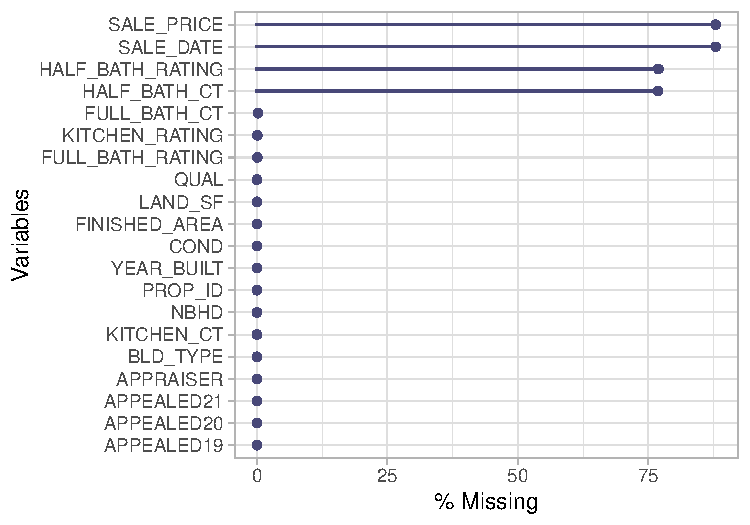
\includegraphics{unnamed-chunk-3-1} 

}

\caption{Proportion of missing data for each variable in the housing data. The variables are also ordered by the amount of missingness.}\label{fig:unnamed-chunk-3}
\end{figure}

Next, we looked at the relationship between appeal status and building
type. Initial comparisons between housing styles and appeal rate over
the three years from 2019 to 2021 suggested a notable correlation
between appeal rates and styles conventionally associated with more
affluent lifestyles, most notably contemporary, mansion, and to a lesser
extent Tudor-style houses. The appeal rates for these luxury residences
normally top out around 4.5\%, though 2020 exceeded 20\% in
contemporary-style buildings alone, the three aforementioned categories
combining for well over 40\% of all appeals.

\begin{figure}[H]

{\centering 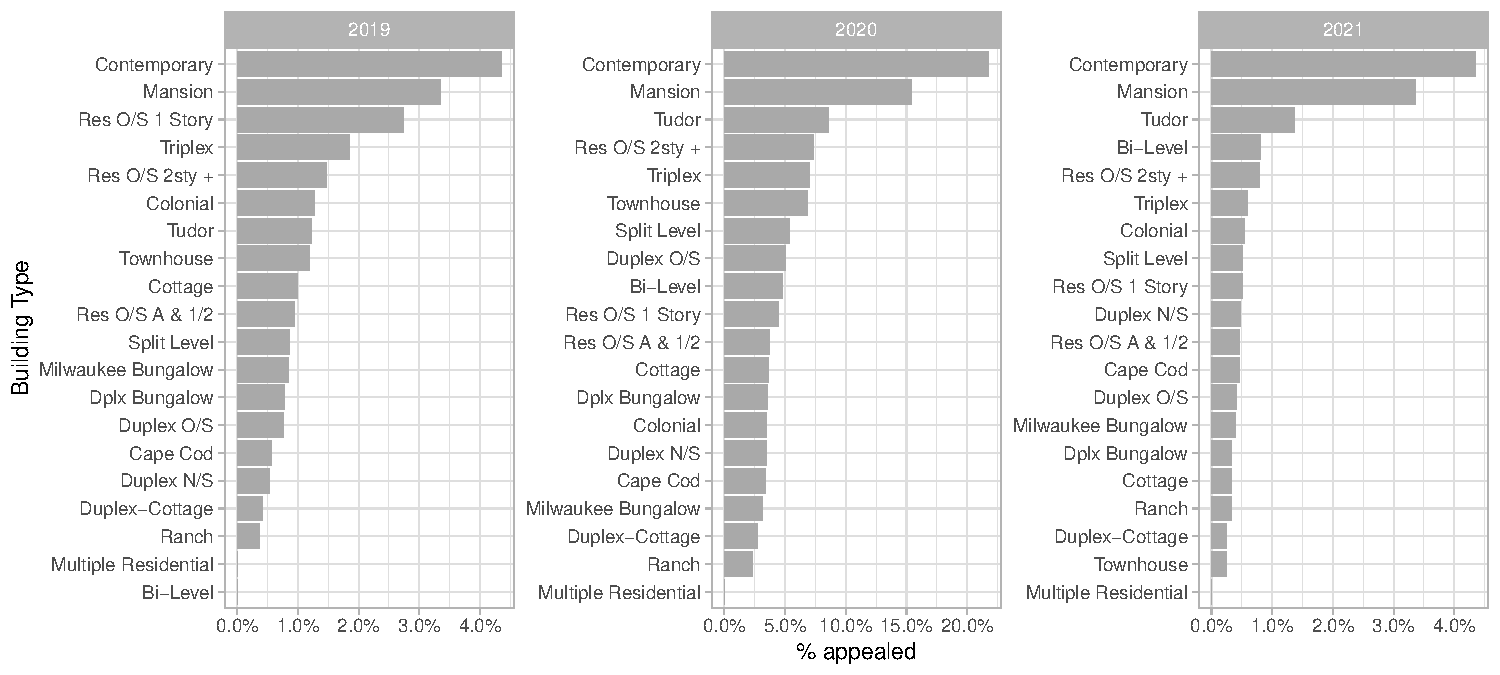
\includegraphics{unnamed-chunk-4-1} 

}

\caption{Property appealed rate for all building types, broken down by year.}\label{fig:unnamed-chunk-4}
\end{figure}

With respect to physical geography, Figure 3 displays the top zip codes
in terms of appeal rate. These zip codes fall into two major location
categories, namely, by the Lake Michigan Shoreline (including downtown),
or situated away from the city near major commuter highways, most
notably interstates 94 and 41. In addition, Figure 4 is a multi-panel
plot of maps showing appeal rates across Milwaukee for the years between
2019 and 2021. This visualization aids the interpretability of our
geographic data, though restricted to the city of Milwaukee. The highest-appealed zip codes, 53212, 53211, and 53207, all fall near
downtown and the Lake Michigan Shore. All in all, property appeal is
undoubtedly tied to geography, thus location variables are likely to be
useful in predicting whether a homeowner appeals their property
assessment.

\begin{figure}[H]

{\centering 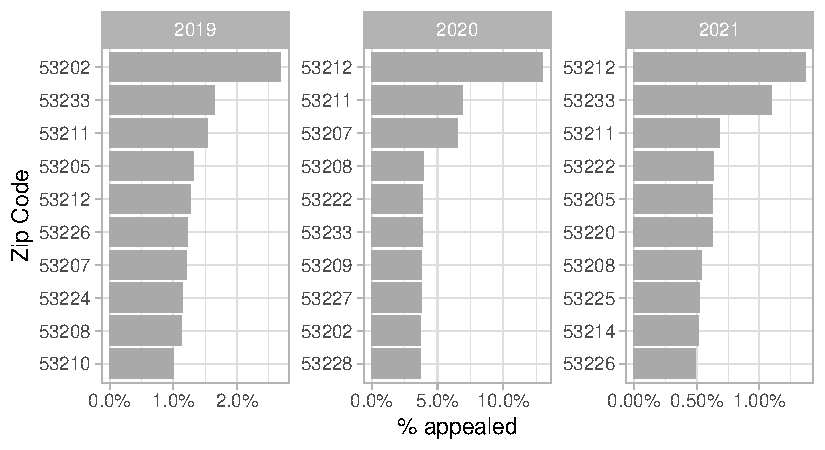
\includegraphics{unnamed-chunk-5-1} 

}

\caption{Top 15 zip codes in Milwaukee with highest property appeal rate for each year between 2019 and 2021.}\label{fig:unnamed-chunk-5}
\end{figure}

\begin{figure}[H]

{\centering 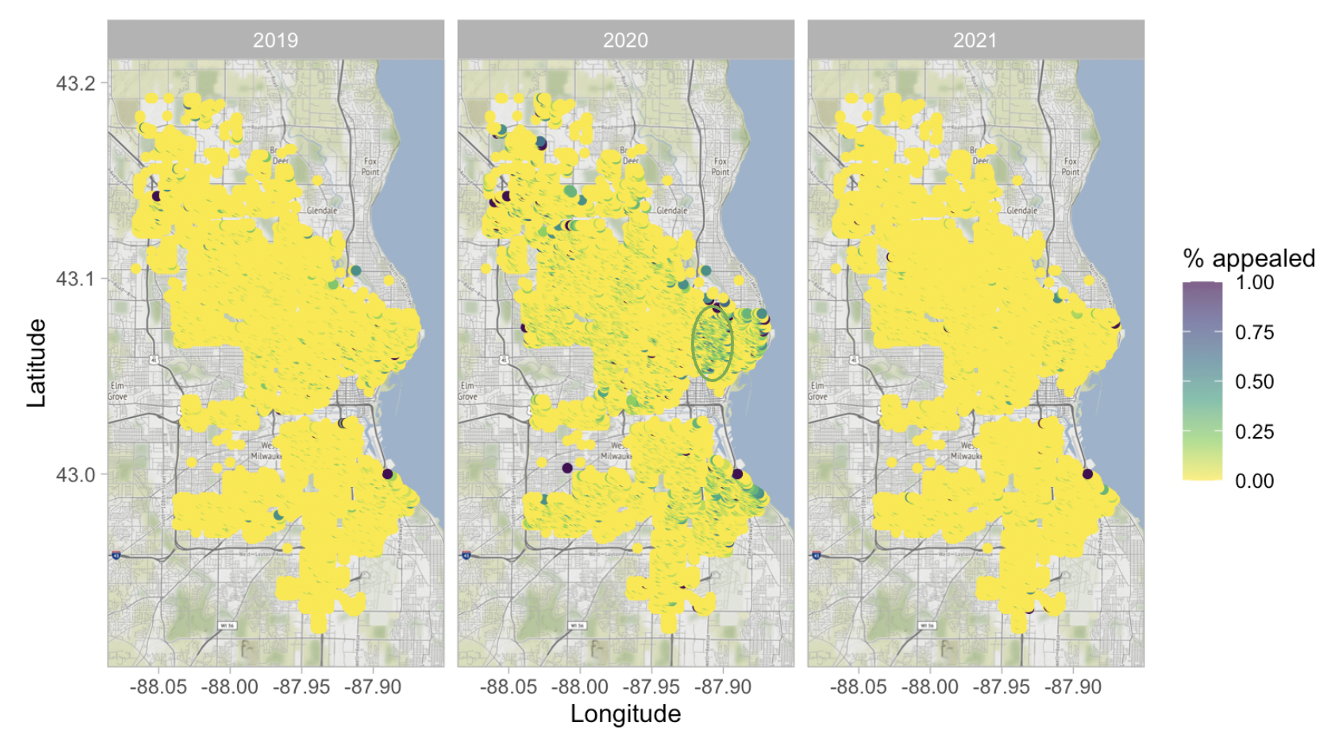
\includegraphics[width=0.9\linewidth]{latlong} 

}

\caption{Map displaying appeal rates across Milwaukee for 2019, 2020, and 2021. The points representing the residential properties are color-coded by appeal rate, where darker colors indicate properties with higher appeal rates. Zip code 53212 is outlined in red in the central map.}\label{fig:unnamed-chunk-6}
\end{figure}

\hypertarget{predictive-models}{%
\section{Predictive Models}\label{predictive-models}}

In this section, we present our modeling strategy for predicting
property assessment appeals for residential properties in the city of
Milwaukee. We explored the performance of different supervised machine
learning approaches on the classification of our target variable, the
appeal status for the tax year 2020.

\hypertarget{data-preparation}{%
\subsection{Data Preparation}\label{data-preparation}}

We started the modeling stage by doing feature engineering to transform
the features in our raw data, making these features more useful in the
machine learning process. For the ordinal categorical variables, we
performed ordinal encoding to the columns representing rating with range
poor to excellent. We converted the levels of these ordinal categorical
predictors into integer values, with 1 representing the lowest level,
poor. In addition, we converted the property quality grade column
(containing values from AA+ to E-) to numeric scores, as suggested by
our client. These are the weight values associated with each quality
grade used by the assessor's office.

In addition, for each nominal categorical covariate, we implemented a
one-hot encoding step. One-hot encoding transforms the predictors into
columns of binary indicators (0 and 1), and for each variable, the
number of new columns should equal the number of the levels belonging to
the initial factor. Moreover, some of the variables in our dataset such
as neighborhood, zip code, and building type contain rare categories (in
one extreme case, a zip code partially outside the city of Milwaukee
contained one appeal out of four total properties, overinflating its
significance), so we decided to lump together the infrequently occurring
levels in each of those factors into another level. Finally, we
considered a natural log transformation for the continuous variables
finished area and land in square feet.

\hypertarget{models}{%
\subsection{Models}\label{models}}

The first model we considered was a LASSO penalized logistic regression
model (Tibshirani, 1996), which is short for Least Absolute Shrinkage
and Selection Operator. LASSO involves penalizing the absolute magnitude
of the regression coefficients, which is commonly known as the
\(\ell_1\) penalty. For our data, LASSO proved a good initial method for
two reasons: relatively easy interpretability and, more importantly, it
handles high dimensional and sparse data well. The LASSO algorithm was
implemented in \texttt{R} using the package \texttt{glmnet} (Friedman et
al., 2010) and \texttt{tidymodels} framework (Kuhn \& Wickham, 2020),
where the error regularization penalty was chosen from model training
via cross-validation.

In addition, we used gradient boosted trees using the popular eXtreme
Gradient Boosting (XGBoost) method (Chen \& Guestrin, 2016) as our
second model. XGBoost has the benefits of being able to scale well with
large, high-dimensional, and sparse data, as well as extremely fast
implementation. In general, gradient boosting goes through cycles to
iteratively add models into an ensemble. The first step is to initialize
the ensemble by creating a single (naive) model. Then the cycle begins,
as the current ensemble is utilized to make predictions, which are then
used to compute a loss function. Based on this loss function result, a
new model is fitted and added to the ensemble. In particular, model
parameters are determined using gradient descent so that adding the new
model to the ensemble will produce a lower loss. Finally, this new model
is added to the ensemble, and then the process is repeated. The XGBoost
method was implemented in \texttt{R} using the package \texttt{xgboost}
(Chen et al., 2021) and \texttt{tidymodels} framework, where tuning via
cross-validation was used to determine the best set of model
hyperparameters.

\hypertarget{model-evaluation}{%
\subsection{Model Evaluation}\label{model-evaluation}}

For both LASSO and XGBoost models, we first partitioned the data using a
70-30 train-test split ratio. Furthermore, a 5-fold cross-validation was
implemented to train each model; and to evaluate the performance of the
classifiers, we used the area under the receiver operating
characteristic curve (AUC) as our evaluation metric.

Figure 5 shows the ROC curve for our LASSO and XGBoost classification
performances on the test data set. We found that a penalty of
\(0.000339\) gave us the best LASSO model in terms of AUC. We used this
LASSO model to get the predicted probability values for property appeal
on the test set and achieved an AUC value of \(0.752\).

For the XGBoost algorithm, we considered various hyperparameters
associated with model complexity, randomness, and step size as tuning
parameters. In terms of model complexity, the optimal combination of
parameters consisted of 411 trees, 5 minimum node data points required
for further splitting, and a subsample ratio of 0.5. As for randomness,
the model selected 13 as the optimal number of randomly sampled
predictors. Finally, we obtained a learning rate of 0.0184 which
determines the step size. The corresponding AUC value for our XGBoost
model on the test set is \(0.771\).

\begin{figure}[H]

{\centering 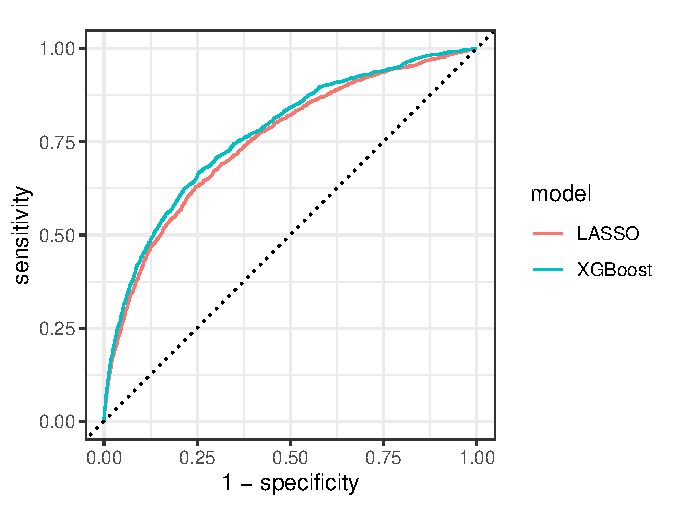
\includegraphics{unnamed-chunk-7-1} 

}

\caption{Receiver operating characteristic curve comparing LASSO and XGBoost classification performances on the test set.}\label{fig:unnamed-chunk-7}
\end{figure}

\hypertarget{other-models}{%
\subsection{Other Models}\label{other-models}}

After fitting two machine learning models, we wanted to look into other
ways of improving our predictions. One particular problem we have with
our dataset is that there is a class imbalance issue with our response
variable, the appeal status in 2020. Specifically, only 3.6\% of
observations had an appeal status of ``yes'' and for the remaining
96.4\%, there was not an appeal (see Table 1). In order to deal with imbalance
classification and possibly improve our performance, we considered SMOTE
(Chawla et al., 2002), an oversampling and data augmentation technique,
short for Synthetic Minority Oversampling Technique. SMOTE works by
selecting candidates that are close to the minority class in the feature
space. In particular, the minority class is oversampled by taking each
observation and introducing synthetic examples along the line segments
joining any or all of their \(k\) nearest neighbors.

We applied the SMOTE technique via the \texttt{themis} package
(Hvitfeldt, 2021) in \texttt{R}. To generate the new examples of the
minority class, we used a default value of \(5\) nearest neighbors and a
majority-to-minority oversampling ratio of \(0.2\). This ratio means the
minority levels would have \(1/5\) as many rows as the majority level as
a result of oversampling. After processing the data, we fed this less
imbalanced data into both LASSO and XGBoost models. However, the AUC
values did not improve for each of the methods. Moreover, further
examination led us to the conclusion that the SMOTE models suffered from
overfitting, failing to produce better results than the previous two
trained models.

\hypertarget{feature-importance}{%
\subsection{Feature Importance}\label{feature-importance}}

After fitting the classification models, we examined the importance of
the features in the data to the model's prediction using the SHAP
(Lundberg \& Lee, 2017) method for model explainability. The name SHAP
comes from Shapley values (Shapley, 1951), an idea from game theory
which describes the average marginal contribution of a player across all
possible coalitions in a game. In a prediction setting, a game can
represent a prediction task for an observation. The players in a game
are feature values associated with each observation that collaborate to
receive a gain or payout, or predict a certain value. The gain or payout
is the difference between the predicted value for a single observation
and the average prediction for all observations.

Since the XGBoost method gave us the best classification results, we
decided to look into variable importance scores for this model. Figure 6
is a bar graph displaying the top 15 features by importance from the
XGBoost model. In addition, Figure 7 is a beeswarm summary plot showing
how the top 15 features in the data impact the XGBoost model's output.
The four features contributing the most to the prediction of property appeal
status were longitude, finished area, whether the house belongs to zip
code 53212, and the year built. Each of these features changes the
predicted absolute appeal probability on average by at least 7.5
percentage points, as illustrated by Figure 6. In addition, the SHAP
beeswarm summary plot indicates that high feature values for longitude,
finished area, zip code 53212, and year built are associated with a
higher probability of appeal. In context, houses that are more likely to
appeal are those located further to the east, with higher total finished
area, belonging to zip code 53212, and were built in a more recent year.

\begin{figure}[H]

{\centering 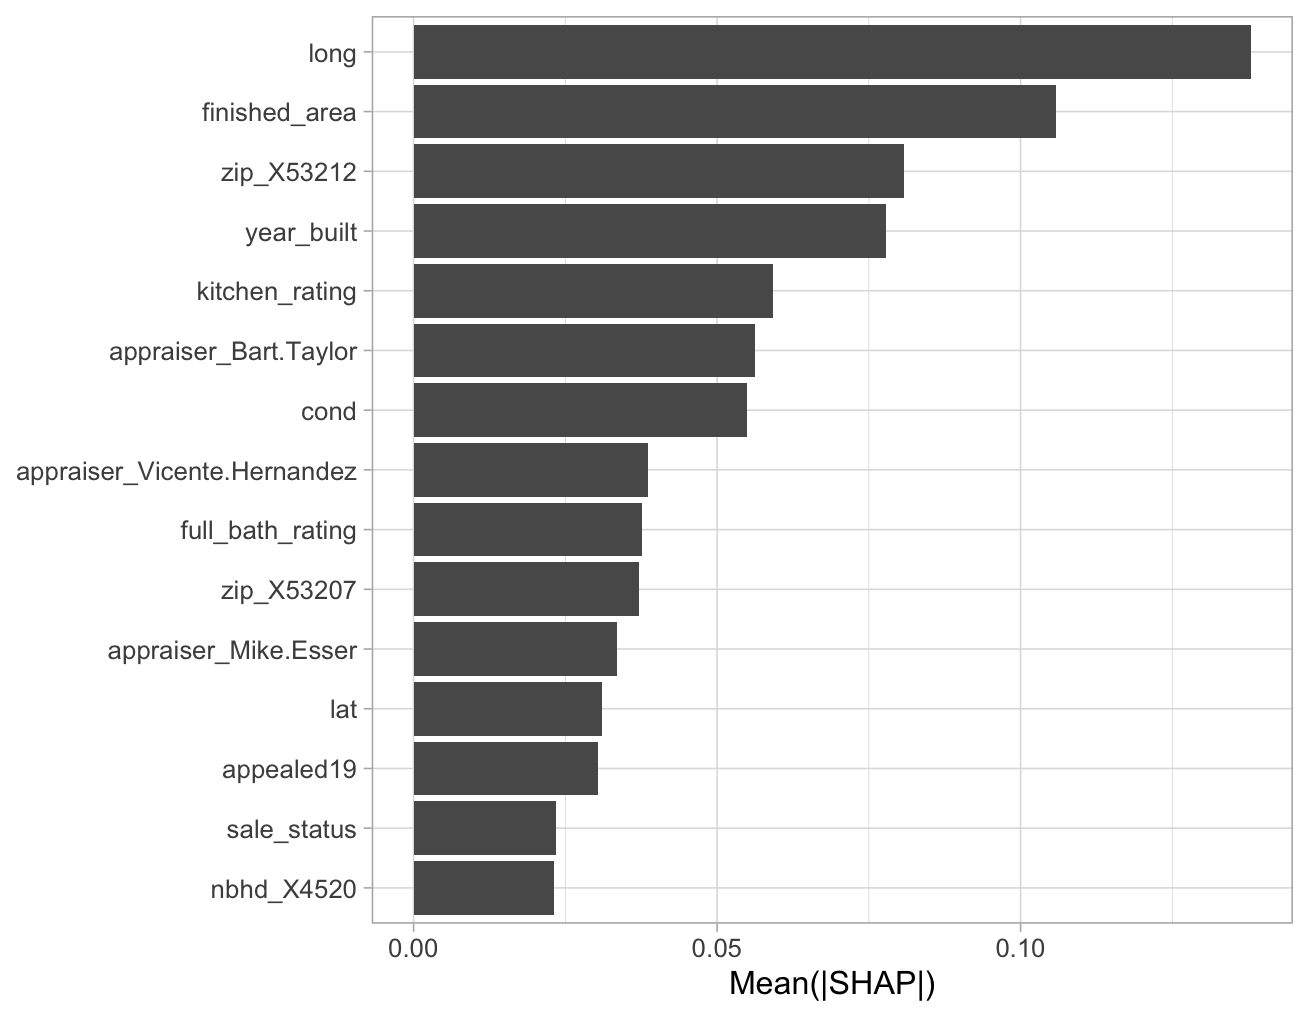
\includegraphics[width=0.7\linewidth]{shapbar} 

}

\caption{Bar graph of top 15 features by importance for the XGBoost model. SHAP feature importance was measured as the mean absolute Shapley values.}\label{fig:unnamed-chunk-8}
\end{figure}

\begin{figure}[H]

{\centering 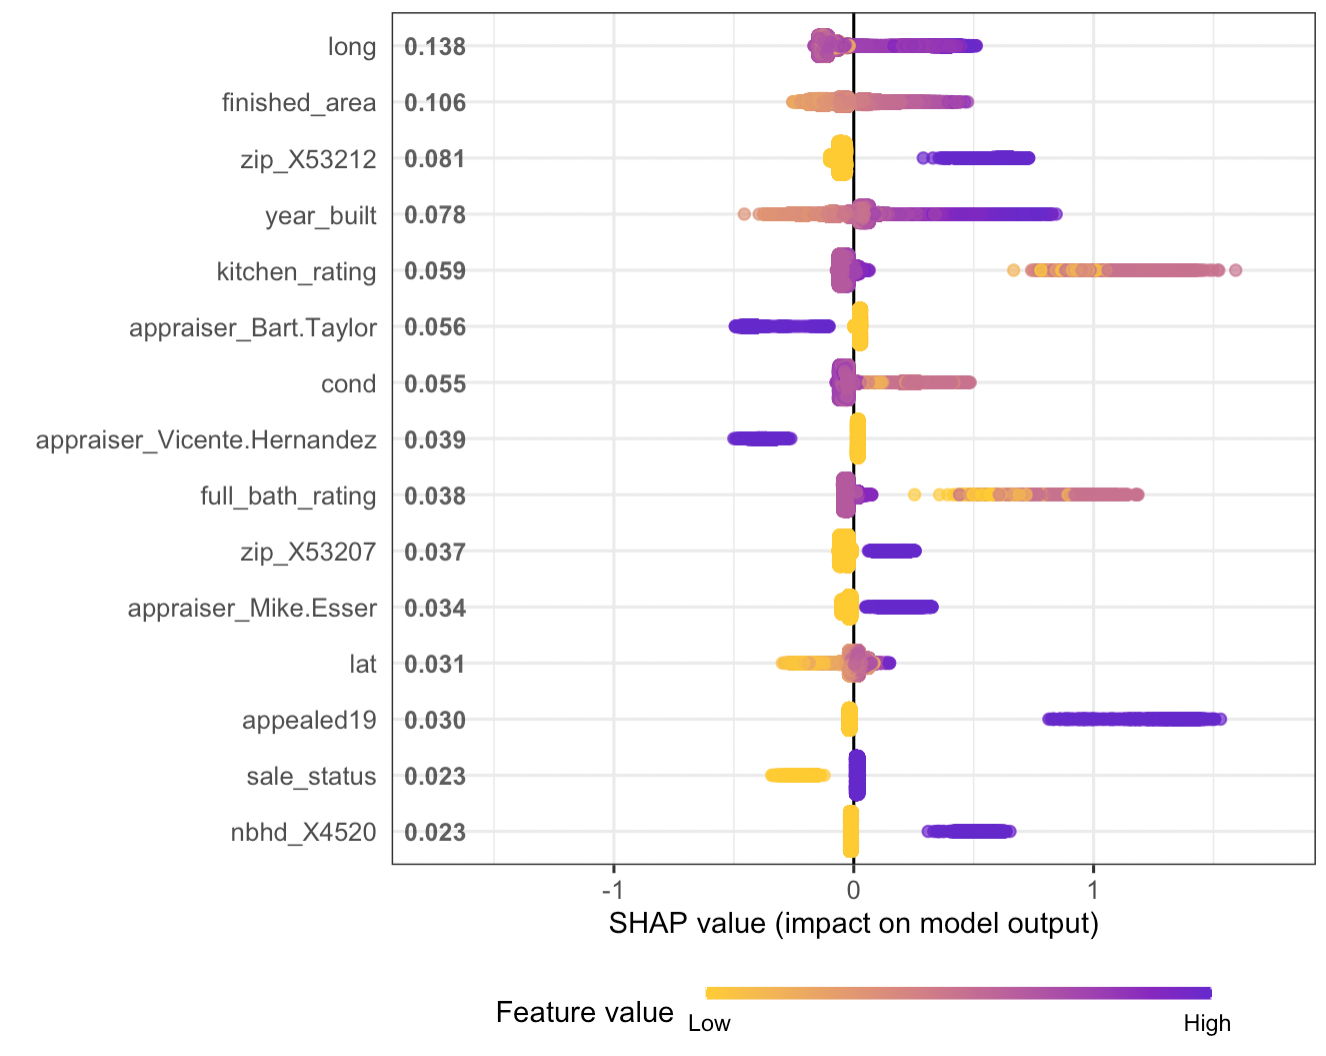
\includegraphics[width=0.72\linewidth]{shapbees} 

}

\caption{Beeswarm plot of top 15 features by importance for the XGBoost model. The summary plot combines feature importance with feature effects, where each dot represents a Shapley value for a feature and an instance. The color represents feature value from low to high.}\label{fig:unnamed-chunk-9}
\end{figure}

\hypertarget{conclusion-and-discussion}{%
\section{Conclusion and Discussion}\label{conclusion-and-discussion}}

This report investigated trends and proposed methodologies for
predicting if a particular property is likely to appeal its valuation
assessment. After considering two supervised machine learning methods, LASSO logistic regression and XGBoost,
it was found that the XGBoost classification
technique performs the best with respect to AUC values. Morever, it was determined from our XGBoost model that 
the variables with the greatest contributions to the prediction of property assessment appeals are location (longitude and zip code 53212), year built, and finished area.

Any future application of this methodology would be wise to incorporate
the context of previous homeownership appeals. In Chicago, only two
hours south of Milwaukee, housing appeals are widely associated with
systematic race-based price devaluation (Moore, 2021), thus adding and
prioritizing a new motive of recouping lost property value. However,
configuring the model to suit more generalized data dating back to
before the 2008 housing crisis for a longitudinal analysis could prove
very beneficial when attempting to predict long-term housing market
trends.

\hypertarget{supplementary-material}{%
\section*{Supplementary Material}\label{supplementary-material}}
\addcontentsline{toc}{section}{Supplementary Material}

All materials related to this manuscript are publicly available on
GitHub at \newline \url{https://github.com/qntkhvn/milwaukee-appeal}. In
addition, source code for a Shiny app for visualizing the predicted
probabilities of appeal for properties in the city of Milwaukee can be
found in the GitHub repository. We chose not to deploy the Shiny app to
an open source Shiny server due to sensitive information regarding
property location, address, and appraiser.

\hypertarget{references}{%
\section*{References}\label{references}}
\addcontentsline{toc}{section}{References}

\hypertarget{refs}{}
\begin{CSLReferences}{1}{0}
\leavevmode\vadjust pre{\hypertarget{ref-tidygeocoder}{}}%
Cambon, J., Hernangómez, D., Belanger, C., \& Possenriede, D. (2021).
Tidygeocoder: An r package for geocoding. \emph{Journal of Open Source
Software}, \emph{6}(65), 3544. \url{https://doi.org/10.21105/joss.03544}

\leavevmode\vadjust pre{\hypertarget{ref-smote}{}}%
Chawla, N. V., Bowyer, K. W., Hall, L. O., \& Kegelmeyer, W. P. (2002).
SMOTE: Synthetic minority over-sampling technique. \emph{J. Artif. Int.
Res.}, \emph{16}(1), 321--357.

\leavevmode\vadjust pre{\hypertarget{ref-xgpaper}{}}%
Chen, T., \& Guestrin, C. (2016). XGBoost: A scalable tree boosting
system. \emph{Proceedings of the 22nd ACM SIGKDD International
Conference on Knowledge Discovery and Data Mining}, 785--794.
\url{https://doi.org/10.1145/2939672.2939785}

\leavevmode\vadjust pre{\hypertarget{ref-xgpackage}{}}%
Chen, T., He, T., Benesty, M., Khotilovich, V., Tang, Y., Cho, H., Chen,
K., Mitchell, R., Cano, I., Zhou, T., Li, M., Xie, J., Lin, M., Geng,
Y., \& Li, Y. (2021). \emph{Xgboost: Extreme gradient boosting}.
\url{https://CRAN.R-project.org/package=xgboost}

\leavevmode\vadjust pre{\hypertarget{ref-glmnet}{}}%
Friedman, J., Hastie, T., \& Tibshirani, R. (2010). Regularization paths
for generalized linear models via coordinate descent. \emph{Journal of
Statistical Software}, \emph{33}(1), 1--22.
\url{https://www.jstatsoft.org/v33/i01/}

\leavevmode\vadjust pre{\hypertarget{ref-themis}{}}%
Hvitfeldt, E. (2021). \emph{Themis: Extra recipes steps for dealing with
unbalanced data}. \url{https://CRAN.R-project.org/package=themis}

\leavevmode\vadjust pre{\hypertarget{ref-tidymodels}{}}%
Kuhn, M., \& Wickham, H. (2020). \emph{Tidymodels: A collection of
packages for modeling and machine learning using tidyverse principles.}
\url{https://www.tidymodels.org}

\leavevmode\vadjust pre{\hypertarget{ref-shap}{}}%
Lundberg, S. M., \& Lee, S.-I. (2017). A unified approach to
interpreting model predictions. \emph{Proceedings of the 31st
International Conference on Neural Information Processing Systems},
4768--4777.

\leavevmode\vadjust pre{\hypertarget{ref-chicago}{}}%
Moore, N. (2021). \emph{Racial inequality in how chicago-area homes are
valued is increasing}.
\url{https://www.wbez.org/stories/racial-inequality-in-how-chicago-area-homes-are-valued-is-increasing/241643ab-6cba-4646-9660-af4f26acc6d8}

\leavevmode\vadjust pre{\hypertarget{ref-rcite}{}}%
R Core Team. (2021). \emph{R: A language and environment for statistical
computing}. R Foundation for Statistical Computing.
\url{https://www.R-project.org/}

\leavevmode\vadjust pre{\hypertarget{ref-shapley}{}}%
Shapley, L. S. (1951). \emph{Notes on the n-person game - {I}:
Characteristic-point solutions of the four-person game}. RAND
Corporation. \url{https://doi.org/10.7249/RM0656}

\leavevmode\vadjust pre{\hypertarget{ref-lassopaper}{}}%
Tibshirani, R. (1996). Regression shrinkage and selection via the lasso.
\emph{Journal of the Royal Statistical Society (Series B)}, \emph{58},
267--288.

\end{CSLReferences}

\end{document}
